\section{Errors and Exceptions}

\begin{frame}[fragile]{Syntax Errors, Indentation Errors}
Errors while parsing: \alert{Program doesn't get executed}. E.g.: 
\begin{itemize}
\item Mismatched or missing parenthesis
\item Missing or misplaced semicolons, colons, commas
\item Indentation errors
\end{itemize}
\begin{lstlisting}[style=Python]
print "I'm running..."
def add(a, b)
   return a + b
\end{lstlisting}
\begin{lstlisting}[style=Shell]
$ ./add.py
  File "add.py", line 2
    def add(a, b)
                ^
SyntaxError: invalid syntax
\end{lstlisting} %$
\end{frame}

\begin{frame}[fragile]{Exceptions}
Exceptions occur at \alert{runtime}:
\begin{lstlisting}[style=Python]
import math
print "I'm running..."
math.foo()
\end{lstlisting}
\begin{lstlisting}[style=Shell]
$ ./test.py
I'm running...
Traceback (most recent call last):
  File "test.py", line 3, in ?
    math.foo()
AttributeError: 'module' object has no 
attribute 'foo'
\end{lstlisting} %$
\end{frame}

\begin{frame}[fragile]{Handling Exceptions}
\begin{lstlisting}[style=Python]
try:
    s = raw_input("Enter a number: ")
    number = float(s)
except ValueError:
    print "That's not a number!"
\end{lstlisting}
\begin{itemize}
\item \lstinline{except} block is executed when the code in the code in the \lstinline{try}-Block throws an according exception
\item afterwards, the program continues normally
\item unhandled exceptions force the program to exit.
\end{itemize}
Handling different kinds of exceptions:
\begin{lstlisting}[style=Python]
except (ValueError, TypeError, NameError):
\end{lstlisting}
\end{frame}

\begin{frame}[fragile]{Handling Exceptions}
\begin{lstlisting}[style=Python]
try:
    s = raw_input("Enter a number: ")
    number = 1/float(s)
except ValueError:
    print "That's not a number!"
except ZeroDivisionError:
    print "You can't divide by zero!"
except:
    print "Oops, what's happened?"
\end{lstlisting}
\begin{itemize}
\item Several \lstinline{except} statements for different exceptions
\item Last \lstinline{except} can be used without specifying the kind of exception: Catches all remaining exceptions
\begin{itemize}
\item Careful: Can mask unintended programming errors!
\end{itemize}
\end{itemize}
\end{frame}

\begin{frame}[fragile]{Handling Exceptions}
\begin{itemize}
\item \alert{\texttt{else}} is executed if no exception occurred
\item \alert{\texttt{finally}} is executed \alert{in any} case
\end{itemize}
\begin{lstlisting}[style=Python]
try:
    f = open("spam")
except IOError:
    print "Cannot open file"
else:
    print f.read()
    f.close()
finally:
    print "End of try."
\end{lstlisting}
\end{frame}

\begin{frame}[fragile]{Exception Objects}
Access to exception objects:
\begin{lstlisting}[style=Python]
try:
    f = open("spam")
except IOError, e:
    print e.errno, e.strerror
    print e
\end{lstlisting}
\begin{lstlisting}[style=Shell]
$ python test.py
2 No such file or directory
[Errno 2] No such file or directory: 'spam'
\end{lstlisting}%$
\end{frame}

\begin{frame}{Exceptions in Function Calls}
\begin{figure}
\centering
\only<1>
{
  \begin{tikzpicture}
  \draw [black] (0, 0.2) node {draw()};
  \draw [white, ->] (0, 0) arc(180:270:15pt) node[anchor=west] {rectangle()};
  \draw [white, ->] (1.5, -0.7) arc(180:270:15pt) 
                    -- (2.5, -1.23) node[anchor=west] {line()};
  \draw [white] (4.6, -1.23) node {Exception!};
  \draw [white, ->] (4.5, -1.0) arc(0:90:15pt) -- (2.8, -0.47);
  \draw [white, ->] (2.6, -0.3) arc(0:90:15pt) -- (0.8, 0.225);
  \end{tikzpicture}
}

\only<2>
{
  \begin{tikzpicture}
  \draw [black] (0, 0.2) node {draw()};
  \draw [black, ->] (0, 0) arc(180:270:15pt) node[anchor=west] {rectangle()};
  \draw [white, ->] (1.5, -0.7) arc(180:270:15pt) 
                    -- (2.5, -1.23) node[anchor=west] {line()};
  \draw [white] (4.6, -1.23) node {Exception!};
  \draw [white, ->] (4.5, -1.0) arc(0:90:15pt) -- (2.8, -0.47);
  \draw [white, ->] (2.6, -0.3) arc(0:90:15pt) -- (0.8, 0.225);
  \end{tikzpicture}
}

\only<3>
{
  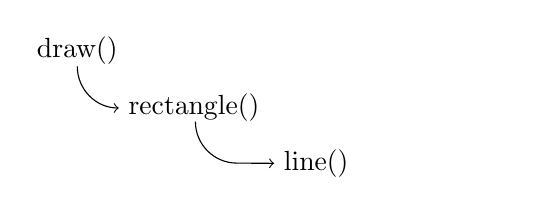
\begin{tikzpicture}
  \draw [black] (0, 0.2) node {draw()};
  \draw [black, ->] (0, 0) arc(180:270:15pt) node[anchor=west] {rectangle()};
  \draw [black, ->] (1.5, -0.7) arc(180:270:15pt) 
                    -- (2.5, -1.23) node[anchor=west] {line()};
  \draw [white] (4.6, -1.23) node {Exception!};
  \draw [white, ->] (4.5, -1.0) arc(0:90:15pt) -- (2.8, -0.47);
  \draw [white, ->] (2.6, -0.3) arc(0:90:15pt) -- (0.8, 0.225);
  \end{tikzpicture}
}

\only<4>
{
  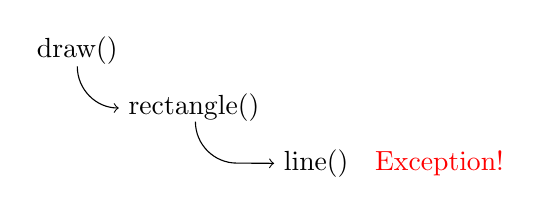
\begin{tikzpicture}
  \draw [black] (0, 0.2) node {draw()};
  \draw [black, ->] (0, 0) arc(180:270:15pt) node[anchor=west] {rectangle()};
  \draw [black, ->] (1.5, -0.7) arc(180:270:15pt) 
                    -- (2.5, -1.23) node[anchor=west] {line()};
  \draw [red] (4.6, -1.23) node {Exception!};
  \draw [white, ->] (4.5, -1.0) arc(0:90:15pt) -- (2.8, -0.47);
  \draw [white, ->] (2.6, -0.3) arc(0:90:15pt) -- (0.8, 0.225);
  \end{tikzpicture}
}

\only<5>
{
  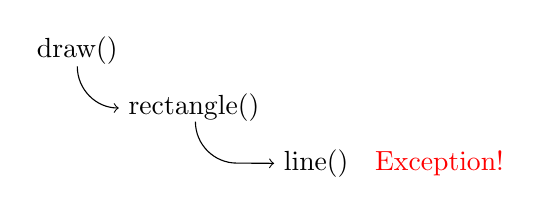
\begin{tikzpicture}
  \draw [black] (0, 0.2) node {draw()};
  \draw [black, ->] (0, 0) arc(180:270:15pt) node[anchor=west] {rectangle()};
  \draw [black, ->] (1.5, -0.7) arc(180:270:15pt) 
                    -- (2.5, -1.23) node[anchor=west] {line()};
  \draw [red] (4.6, -1.23) node {Exception!};
  \draw [white, ->] (4.5, -1.0) arc(0:90:15pt) -- (2.8, -0.47);
  \draw [white, ->] (2.6, -0.3) arc(0:90:15pt) -- (0.8, 0.225);
  \end{tikzpicture}
}

\only<6>
{
  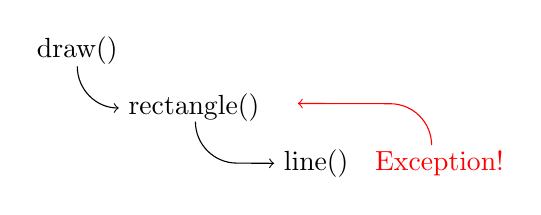
\begin{tikzpicture}
  \draw [black] (0, 0.2) node {draw()};
  \draw [black, ->] (0, 0) arc(180:270:15pt) node[anchor=west] {rectangle()};
  \draw [black, ->] (1.5, -0.7) arc(180:270:15pt) 
                    -- (2.5, -1.23) node[anchor=west] {line()};
  \draw [red] (4.6, -1.23) node {Exception!};
  \draw [red, ->] (4.5, -1.0) arc(0:90:15pt) -- (2.8, -0.47);
  \draw [white, ->] (2.6, -0.3) arc(0:90:15pt) -- (0.8, 0.225);
  \end{tikzpicture}
}

\only<7>
{
  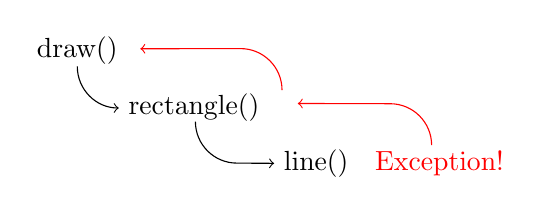
\begin{tikzpicture}
  \draw [black] (0, 0.2) node {draw()};
  \draw [black, ->] (0, 0) arc(180:270:15pt) node[anchor=west] {rectangle()};
  \draw [black, ->] (1.5, -0.7) arc(180:270:15pt) 
                    -- (2.5, -1.23) node[anchor=west] {line()};
  \draw [red] (4.6, -1.23) node {Exception!};
  \draw [red, ->] (4.5, -1.0) arc(0:90:15pt) -- (2.8, -0.47);
  \draw [red, ->] (2.6, -0.3) arc(0:90:15pt) -- (0.8, 0.225);
  \end{tikzpicture}
}
\end{figure}
\begin{itemize}
\item<1-> Function calls another function.
\item<4-> That function raises an exception.
\item<5-> Is exception handled?
\item<6-> No: Pass exception to calling function.
\end{itemize}
\end{frame}

\begin{frame}[fragile]{Raising Exceptions}
Passing exceptions on:
\begin{lstlisting}[style=Python]
try:
    f = open("spam")
except IOError:
    print "Problem while opening file!"
    raise
\end{lstlisting}
\vspace{3mm}
Raising exceptions:
\begin{lstlisting}[style=Python]
def gauss_solver(matrix):
    # Important code
    raise ValueError("Singular matrix")
\end{lstlisting}
\end{frame}


\begin{frame}[fragile]{Exceptions vs. Checking Values Beforehand}
\onslide<1->
Exceptions are preferable!

\begin{lstlisting}
def square(x):
    if type(x) == int or type(x) == float:
        return x ** 2
    else:
        return None
\end{lstlisting}
Bad!

\onslide<2->
\begin{itemize}
  \item What about other numerical data types (complex numbers, own data types)? Better: Try to compute the power and catch possible exceptions! $\rightarrow$ \alert{Duck-Typing}

  \item Caller of a function might forget to check return values for validity. Better: Raise an exception!
\end{itemize}
\end{frame}


\begin{frame}[fragile]{The \texttt{with} Statement}
Some objects offer context management, which provides a more convenient way to write \lstinline{try ... finally} blocks:
\begin{lstlisting}
with open("test.txt") as f:
    for line in f:
        print line
\end{lstlisting}
After the \lstinline{with} block the file object is guaranteed to be closed properly, no matter what exceptions occurred within the block.\vspace{5mm}

In Python 2.5 this needs the following import:
\begin{lstlisting}
from __future__ import with_statement
\end{lstlisting}
\end{frame}
